\textbf{Beispiel 1}\\ \\
a)\\ \\
Freigeschnittene Massen:
\begin{figure}[h]
 	\centering
 	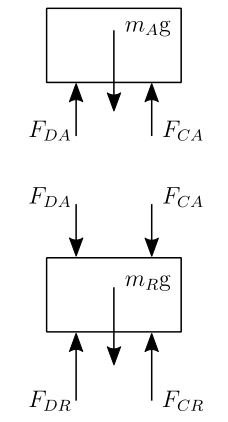
\includegraphics[width= 3cm]{tikz/29_09_2017_1a}
\end{figure}
\newline
Die Berechnungsvorschriften lauten
\begin{align*}
	F_{CA} = c_a(x_R - x_A) & F_{DA} = d_A(v_{RA})(\dot{x}_R - \dot{x}_A) \\
	F_{CR} = c_R(x_U - x_R) & F_{DR} = d_R(\dot{x}_U - \dot{x}_R)
\end{align*}
b)\\ \\
Die Bewegungsgleichungen der Massen kann mithilfe der Implulserhaltung aufgestellt werden und lauten für den Aufbau
\[
	m_A\ddot{x}_A = F_{CA} + F_{DA} - m_Ag
\]
und für das Rad
\[
	m_R\ddot{x}_R = F_{CR} + F_{DR} - F_{CA} - F_{DA} - m_Rg
\]
c)\\ \\
Im stationären Fall lauten die beiden Bewegungsgleichungen
\begin{align*}
	0 &= F_{CA} - m_Ag \\
	0 &= F_{CR} - F_{CA} - m_Rg
\end{align*}
Aus der ersten Gleichung folgt
\[
	F_{CA} = m_Ag
\]
\newpage
\noindent
Nun setzt man dies in die zweite Bewegungsgleichung ein. Das führt dann auf
\begin{align*}
	0 &= F_{CR} - m_Ag - m_Rg \\
	0 &= -c_Rx_R - m_Ag - m_Rg \\
	x_R &= -\frac{(m_A + m_R)g}{c_R}
\end{align*}
Daraus folgt für die andere Auslenkung
\begin{align*}
	F_{CA} = m_Ag &= c_a(x_R - x_A) \\
	m_Ag &= -c_A\left(\frac{(m_A + m_R)g}{c_R} + x_A\right) \\
	-\frac{m_Ag}{c_a} &= \frac{(m_A + m_R)g}{c_R} + x_A \\
	x_A &= -\frac{(m_A + m_R)g}{c_R} - \frac{m_Ag}{c_a} 
\end{align*}
d)\\ \\
Freigeschnittene Radaufhängung:
\begin{figure}[h]
	\centering
	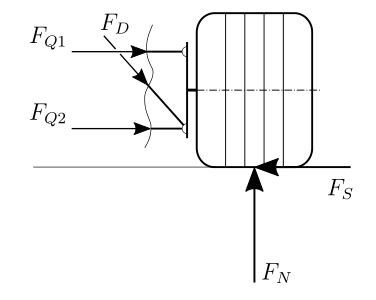
\includegraphics[width= 5cm]{tikz/29_09_2017_1d}
\end{figure}
\newline
e)\\ \\
Der Drehpunkt für die Momentengleichung ist der Schnittpunkt der Stäbe Q2 und D. Die Gleichgewichtsbedingungen für die Radaufhängung lautet daher
\begin{align*}
	\textbf{e}_x &: F_{Q1} + F_{Q2} - F_S + F_D\cos(\alpha) = 0\\
	\textbf{e}_y &: -F_D\sin(\alpha) + F_N\\
	\textbf{e}_z &: -F_{Q1}b - F_Sa + F_Nd
\end{align*}
\newpage
\noindent
Aus diesen Gleichungen können nun die gesuchten Stabkräfte bestimmt werden.
\begin{align*}
	F_D &= \frac{F_N}{\sin(\alpha)} \\
	F_{Q1} &= \frac{F_Nd - F_Sa}{b} = \frac{\frac{F_N}{\sin(\alpha)}d - F_Sa}{b} \\
	0 &= \frac{\frac{F_N}{\sin(\alpha)}d - F_Sa}{b} + F_{Q2} - F_S + \frac{F_N}{\sin(\alpha)}\cos(\alpha) \\
	F_{Q2} &= F_S\left(1 + \frac{a}{b}\right) - F_N\left(\cot(\alpha) + \frac{d}{b}\right)
\end{align*}